\documentclass[a4paper,10pt,landscape,twocolumn]{scrartcl}

%% Settings
\newcommand\problemset{3}
\newcommand\worksession{Tuesday, 26 September 2017}
\newif\ifcomments
\commentsfalse % hide comments
%\commentstrue % show comments

%% Packages
\usepackage[english]{exercises}
\usepackage{wasysym}
\usepackage{graphicx}
\usepackage{hyperref}
\hypersetup{colorlinks=true, urlcolor = blue, linkcolor = blue}
% \usepackage{enumitem}

%% Macros
\usepackage{xspace}

\newcommand{\eps}{\varepsilon}
\newcommand{\ket}[1]{|#1\rangle}
\newcommand{\bra}[1]{\langle#1|}
\newcommand{\inp}[2]{\langle{#1}|{#2}\rangle}
\newcommand{\norm}[1]{\parallel\!#1\!\parallel}
\newcommand{\points}[1]{\marginpar{\textbb{#1 p.}}}
\newtheorem{theorem}{Theorem}
\newtheorem{definition}{Definition}
\newtheorem{proposition}{Proposition}
%\newenvironment{proof}{\noindent {\bf Proof }}{{\hfill $\Box$}\\}

\newcommand{\gen}{\ensuremath{\mathsf{Gen}}\xspace}
\newcommand{\enc}{\ensuremath{\mathsf{Enc}}\xspace}
\newcommand{\dec}{\ensuremath{\mathsf{Dec}}\xspace}
\newcommand{\mac}{\ensuremath{\mathsf{Mac}}\xspace}
\newcommand{\vrfy}{\ensuremath{\mathsf{Vrfy}}\xspace}
\newcommand{\negl}{\ensuremath{\mathsf{negl}}\xspace}
\newcommand{\PrivK}{\ensuremath{\mathsf{PrivK}}\xspace}
\newcommand{\eav}{\ensuremath{\mathsf{eav}}\xspace}

\newcommand{\Z}{\ensuremath{\mathbb{Z}}}
\newcommand{\R}{\ensuremath{\mathbb{R}}}
\newcommand{\N}{\ensuremath{\mathbb{N}}}


\newcommand\floor[1]{\lfloor#1\rfloor}
\newcommand\ceil[1]{\lceil#1\rceil}

% \newcommand{\comment}[1]{{\sf [#1]}\marginpar[\hfill !!!]{!!!}}
\newcommand{\chris}[1]{\comment{\color{blue}Chris: #1}}
\newcommand{\jan}[1]{\comment{\color{magenta}Jan: #1}}


\begin{document}

\problems


\begin{exercise}[Basic properties of PRFs]
The set of all functions from $n$ bits to $\ell$ bits is denoted by
\[ \mathsf{Func}_{n,\ell} := \big\{f:\{0,1\}^n \rightarrow \{0,1\}^{\ell} \big\} \, .
\]
Note that with this definition, we have that $\mathsf{Func}_n$ as defined on page 77 of [KL] is equal to $\mathsf{Func}_{n,n}$.

Let $F:\{0,1\}^n \times \{0,1\}^n \rightarrow \{0,1\}^\ell$ be a pseudorandom function.

\begin{subex}
How many functions are there in $\mathsf{Func}_{n,\ell}$?
\end{subex}

\begin{subex}
How many functions $F_k:\{0,1\}^n \rightarrow \{0,1\}^\ell$ are there if you vary $k$?
\end{subex}

\begin{subex}
Let $h(n,\ell)$ denote the fraction of functions $F_k$ among all functions in $\mathsf{Func_{n,\ell}}$. Argue that $h(n, \ell)$ is a negligible function in $n$. Argue that $h(n,\ell)$ is also negligible in $\ell$.
\end{subex}

\end{exercise}


\begin{exercise}[not PRFs]
Let us assume that $k$ and $x$ are $n$-bit strings. For all of the following constructions, explain why they are not PRFs. Give an explicit description of an efficient attacker that distinguishes the given function from a uniform function $f \in \mathsf{Func}_n$.

\begin{subex}
Let $F_k(x)$ output $k$.
\end{subex}

\begin{subex}
Let $F_k(x)$ output $x$.
\end{subex}

\begin{subex}
Let $F_k(x)$ output $x \oplus k$. Play around as the distinguisher for this function \href{https://staff.fnwi.uva.nl/j.m.czajkowski/game/prf.html}{here} and program a successful distinguisher in \href{https://colab.research.google.com/drive/1uCr-BvOARnlc3qAp2nam2FlxpQBUVMgS}{this notebook}!
\end{subex}

\end{exercise}


\begin{figure}[h]
\center
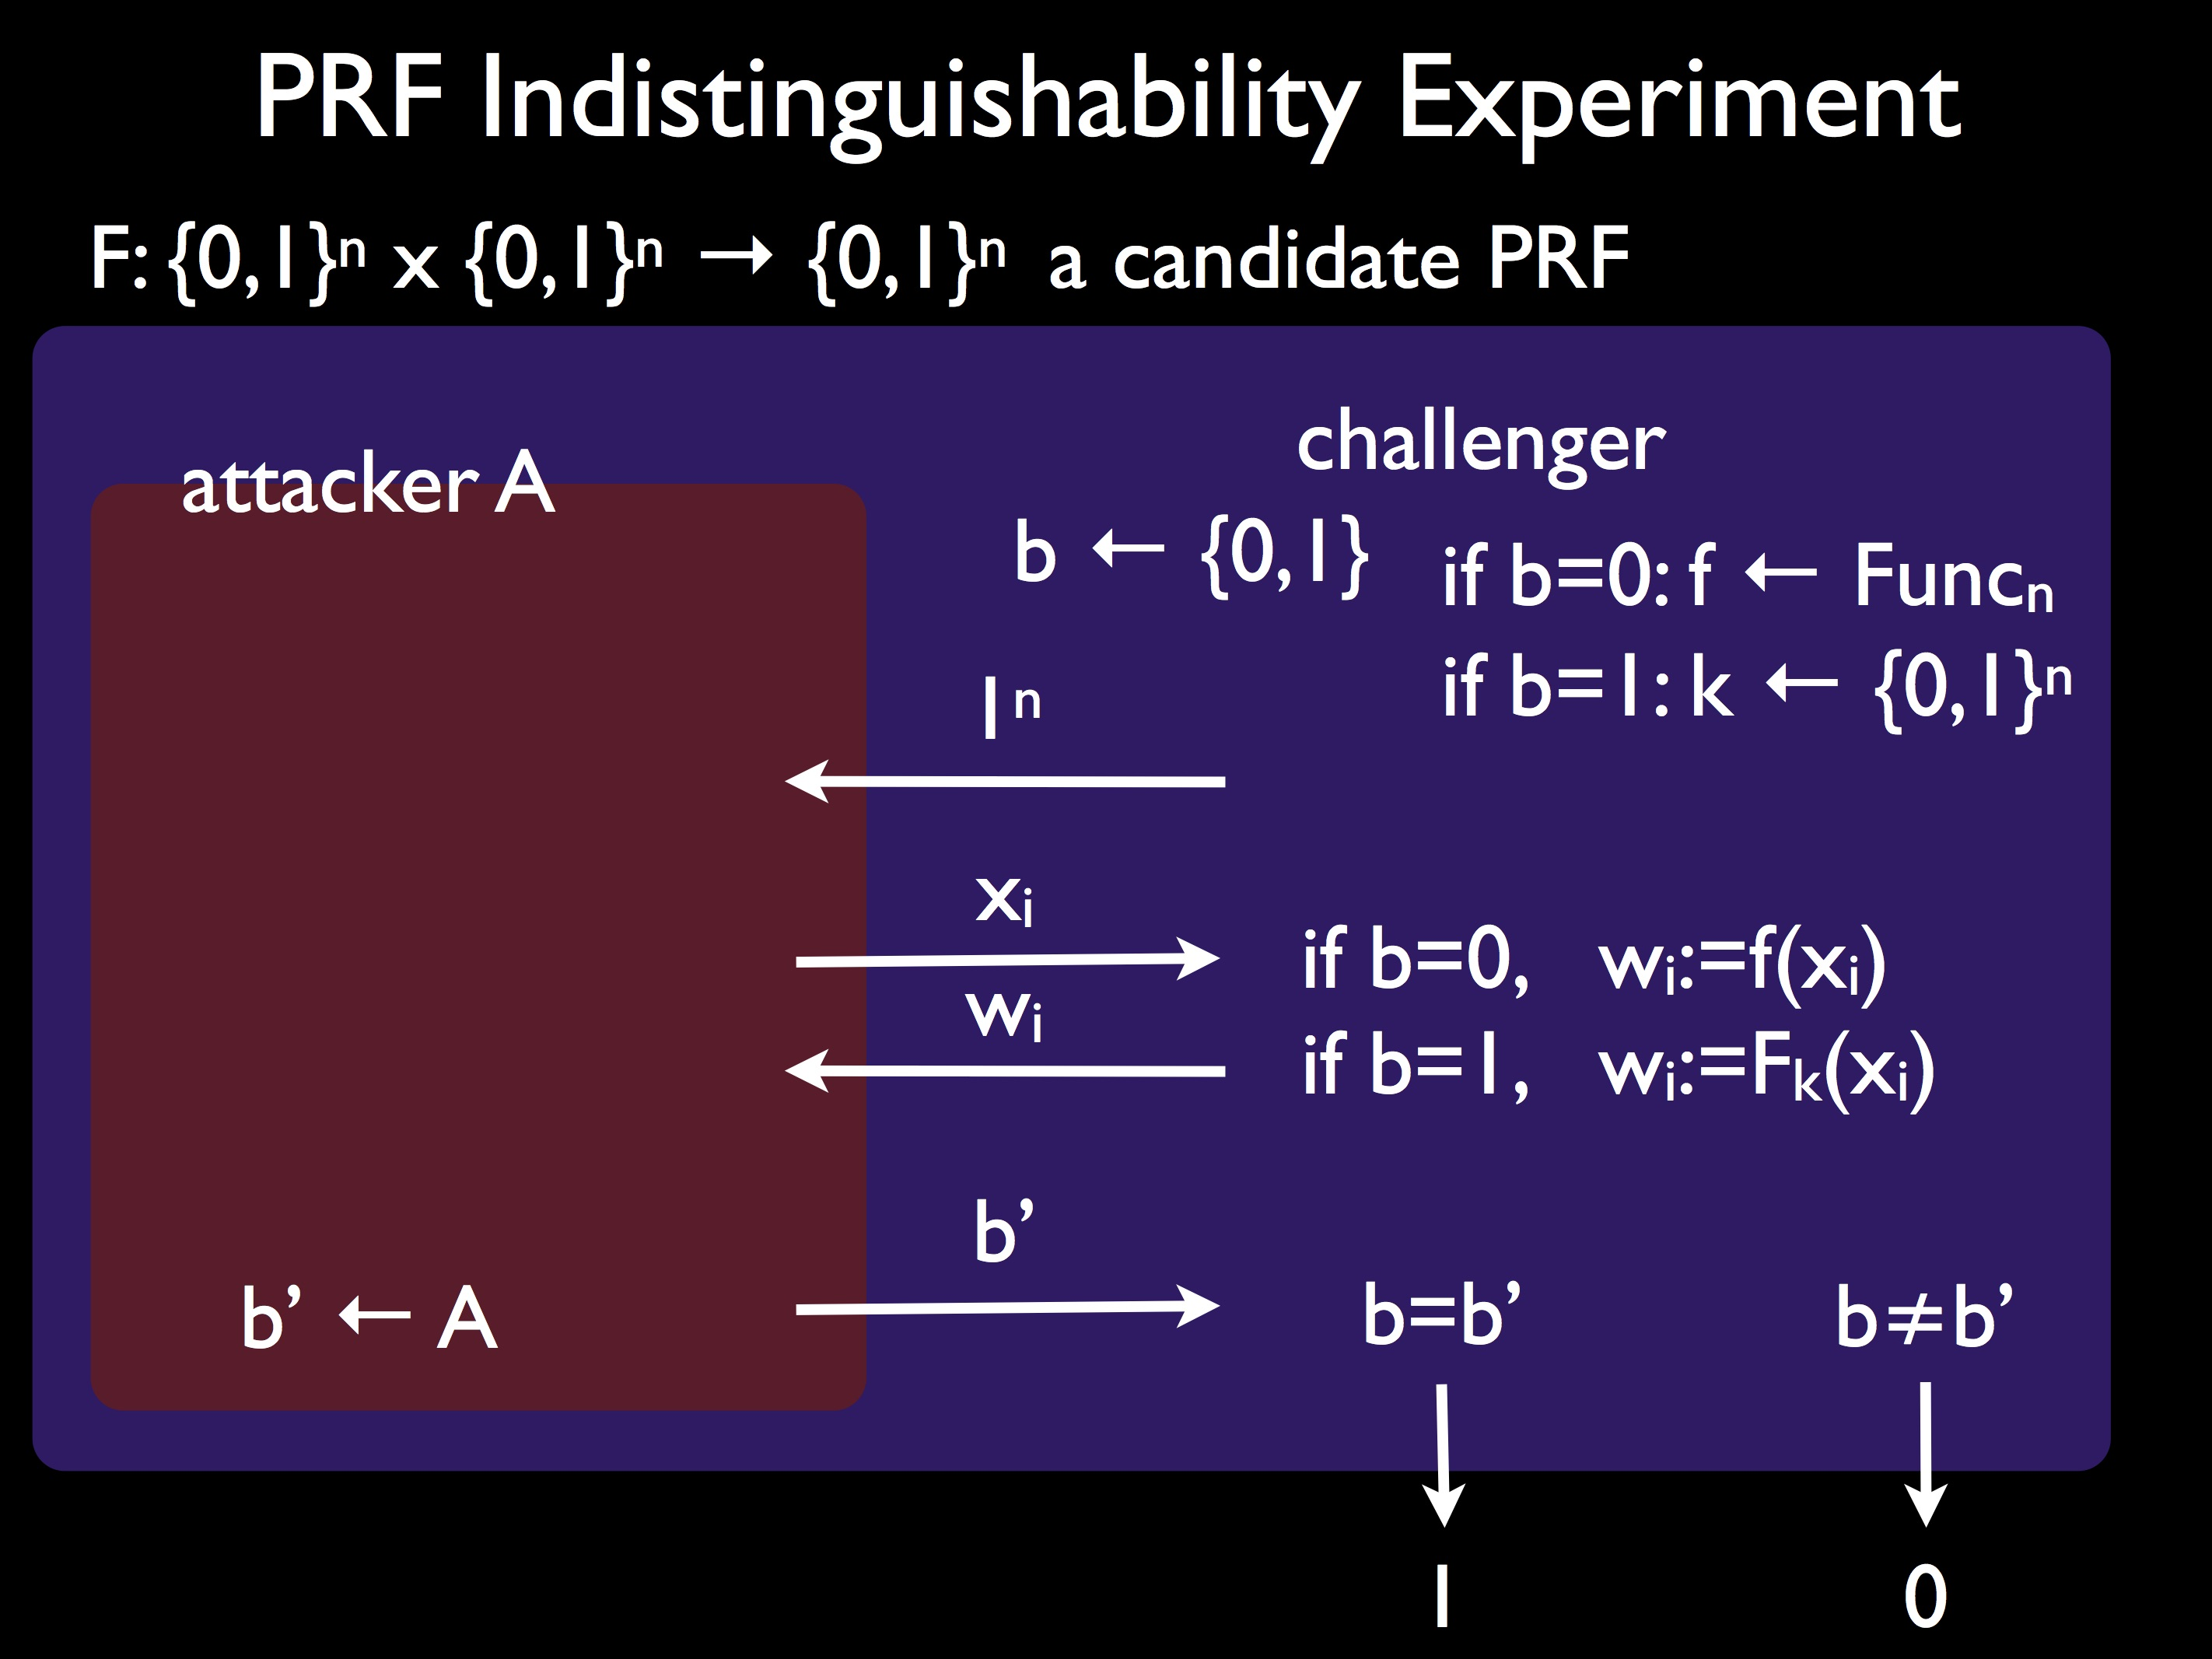
\includegraphics[width=8cm]{PRFExperiment.jpg}
\caption{The $\mathsf{PRF}_{\mathcal{A},F}(n)$ experiment \label{fig}}
\end{figure}



\begin{exercise}[Exercise~3.12]

Let $F$ be a keyed function and consider the following experiment:

\textbf{The PRF indistinguishability experiment
  $\mathsf{PRF}_{\mathcal{A},F}(n)$:}, see also Figure~\ref{fig}:
\textit{
\begin{enumerate}
\item A uniform bit $b \in \{0, 1\}$ is chosen. If $b = 1$ then choose
uniform $k\in \{0, 1\}^n$ .
\item $\mathcal{A}$ is given $1^n$ for input. If $b = 0$ then $\mathcal{A}$ is given access to
a uniform function $f \in \mathsf{Func}_n$ . If $b = 1$ then $\mathcal{A}$ is instead
given access to $F_k(\cdot)$.
\item $\mathcal{A}$ outputs a bit $b'$.
\item The output of the experiment is defined to be 1 if $b' = b$,
and 0 otherwise.
\end{enumerate}
}

We can give an alternative definition of PRFs using this experiment as
follows:

\textbf{Definition: } Let $F:\{0,1\}^* \times \{0,1\}^* \rightarrow \{0,1\}^*$ be an efficient
length-preserving keyed function. F is a \emph{pseudorandom function}
if for all probabilistic polynomial-time attackers $\mathcal{A}$, there is a
negligible function $\negl$ such that:
\[ 
\Pr[\mathsf{PRF}_{\mathcal{A},F}(n) = 1] \leq \frac12 + \negl(n) \, , 
\]
where the probability is taken over the randomness used by
$\mathcal{A}$ and the rnadomness used in the experiment (for choosing
the bit $b$ as well as $f$ and $k$).


Prove that the definition above is equivalent to Definition 3.25.
\end{exercise}


\begin{exercise}[Exercise~3.20 from  $\text{[KL]}$ ]
  Consider a stateful variant of CBC-mode encryption where the sender simply increments the $IV$ by 1 each time a message is encrypted (rather than choosing $IV$ at random each time). Show that the resulting scheme is \emph{not} CPA-secure.
\end{exercise}

\begin{exercise}[Exercise~3.28 from $\text{[KL]}$ ]
Show that the CBC, OFB, and CTR modes of operation do not yield CCA-secure encryption schemes (regardless of $F$). Consider encryptions and decryptions of only single-block messages.
\end{exercise}

\begin{exercise}[Exercise~3.29 from $\text{[KL]}$ ]
  Let $\Pi_1 = (\gen_1,\enc_1, \dec_1)$ and $\Pi_2 = (\gen_2,\enc_2, \dec_2)$ be two encryption schemes for which it is known that at least one is CPA-secure (but you don't know which one). Show how to construct an encryption scheme $\Pi$ that is guaranteed to be CPA-secure as long as at least one of $\Pi_1$ or $\Pi_2$ is CPA-secure. Provide a full proof of your solution.

  \textbf{Hint:} Generate two plaintext messages from the original plaintext so that knowledge of either one reveals nothing about the original plaintext, but knowledge of both enables the original plaintext to be computed.
\end{exercise}



%\begin{bonusexercise}[Exercise~3.14 from $\text{[KL]}$ ]
%Argue that if $F$ is a length-preserving pseudorandom function, then
%$G(s) := F_s(1)\Vert F_s(2)\Vert \cdots \Vert F_s(\ell)$ is a pseudorandom generator with expansion factor $\ell \cdot n$.
%\end{bonusexercise}


\begin{bonusexercise}[Exercise~3.9 from  $\text{[KL]}$ ]
  Prove \emph{unconditionally} the existence of a pseudorandom function $F : \{0,1\}^{n^2} \times \{0,1\}^{\log(n)} \to \{0,1\}^n$.

  \textbf{Hint:} Use the function input as index to select part of the key.
\end{bonusexercise}

\begin{bonusexercise}[Exercise~3.16 from $\text{[KL]}$ ]
  Prove Proposition 3.27:
  \textit{
If $F$ is a pseudorandom permutation and additionally $\ell_{in}(n) \geq n$, then $F$ is also a pseudorandom function.
  }

\textbf{Hint:} Use the results of Appendix A.4.
\end{bonusexercise}

%\begin{bonusexercise}[Exercise~3.26 from $\text{[KL]}$ ]
%  For any function $g : \{0, 1\}^n \to \{0, 1\}^n$ , define $g^{\$} (·)$ to be a probabilistic oracle that, on input $1^n$, chooses uniform $r \in \{0, 1\}^n$ and returns $\langle r, g(r)\rangle$. A keyed function $F$ is a \emph{weak pseudorandom function} if for all PPT algorithms $D$, there exists a negligible function $\mathsf{negl}$ such that:
%  \begin{equation}
%  \left\lvert  \text{Pr}[ D^{F_k^{\$}(.)}(1^n)=1 ]-\text{Pr}[ D^{f^{\$}(.)}(1^n)=1 ]  \right\rvert < \mathsf{negl}(n),
%  \end{equation}
%where $k \in \{0, 1\}^n$ and $f \in \mathsf{Func}_n$ are chosen uniformly.
%\begin{enumerate}[label=(\alph*)]
%\item Prove that if $F$ is pseudorandom then it is weakly pseudorandom.
%\item Let $F'$ be a pseudorandom function, and define
%\begin{equation}
%F_k(x):=\begin{cases}
%    F'_k(x)     & \quad \text{if } x \text{ is even}\\
%    F'_k(x+1)  & \quad \text{if } x \text{ is odd.}
%  \end{cases}
%\end{equation}
%Prove that $F$ is weakly pseudorandom, but \emph{not} pseudorandom.
%\item Is CTR-mode encryption using a weak pseudorandom function necessarily CPA-secure? Does it necessarily have indistinguishable encryptions in the presence of an eavesdropper? Prove your answers.
%
% \textbf{Hint:} Consider CTR-mode using $F$ defined above, show an attack on this encryption scheme.
%\item Prove that Construction 3.30 is CPA-secure if $F$ is a weak pseudorandom function.
%\end{enumerate}
%\end{bonusexercise}


\end{document}
